\chapter{Development}

This chapter will discuss the development of the project. Rather than going into detail how each sprint has been done, it will focus on the main features implemented, how this was achieved and will talk about successes or challenged that were encountered in the development process.

\section{Sprint \#1}

The first sprint of this project was focused in laying the groundwork for the project, which mainly involved setting up the schemas for the ORM that would create the tables for the database, the initial setup of the API endpoints, such as the login and register endpoints, authentication and other security measures, but also setting up the frontend of the project.

\subsection{SQLModel Schemas \& Database creation}

SQLModel played a pivotal role in helping quickly build the database tables. As previously mentioned in~\ref{sec:techstack}, SQLModel is built on top of SQLAlchemy and Pydantic, both being very powerful Python libraries. Pydantic was used to create the schemas that were used both within the backend but also by SQLAlchemy to create the tables in the database. 

Below is an example of a schema that was used to create the User table in the database.

\begin{lstlisting}[language=Python, caption=SQLModel User Schema]
# Base model that contains the field serialiser for date formatting to dd-mm-yyyy and the date field itself
    class DateFormattingModel(SQLModel):
        dob: date | None = None
    
        @field_serialiser('dob')
        def serialise_dob(self, value: date) -> str:
            return value.strftime("%d-%m-%Y")
    
    class User(DateFormattingModel, table=True):
        id: uuid.UUID = Field(default_factory=uuid.uuid4, primary_key=True)
        name: str
        email: EmailStr = Field(index=True, unique=True)
        hashed_password: str
\end{lstlisting}

Similarly, SQLModel (and more specifically Pydantic schemas) could be used to create response/request models that would be used by the endpoints to validate the data that was being sent to or by the API. These schemas did not create tables in the database, but were used to control or validate the data being sent to or from the API.

Below is an example of a SQLModel/Pydantic schema that was used to validate the data that was being sent to the register endpoint.

\begin{lstlisting}[language=Python, caption=SQLModel Auth Schema]
    # User Data model used for login and registration
    class UserAuth(SQLModel):
        email: EmailStr
        password: str
        name: str | None = None # Will only be used for registration

    # User Data model used for most API responses
    class UserPublic(SQLModel):
        id: uuid.UUID
\end{lstlisting}

\subsection{Authentication \& APIs}

As the project was centered around building a PHR system that would deal with sensitive health data, one of the main concerns was the security of the system and its users. 

One of the important choices to make was how to handle the authentication. Based on research on modern authentication methods, the student has identified 4 different ways to handle authentication in the project:

\begin{itemize}
    \item JWT Tokens
    \item OAuth2
    \item Session-based authentication
    \item Using 3rd party authentication services, like Auth0
\end{itemize}

Each method has its own disadvantages and advantages, which will be briefly discussed below.
JWT (JSON Web Tokens) authentication involves generating tokens containing user information for client-side storage \parencite{auth1}. While it requires minimal server-side management, tokens can be vulnerable to XSS and CSRF attacks and cannot be invalidated once created \parencite{auth1, auth2}. The authors recommend using methods like pairs of access and refresh tokens to mitigate these risks, and also to store the tokens in cookies.

Session-based authentication stores session information server-side, using cookies to maintain client sessions \parencite{auth1, auth2}. While cookies can face similar security risks as JWT, they can be secured through flags like HttpOnly and SameSite \parencite{mozilla}. Sessions can be invalidated server-side, providing better security control.

Third-party authentication options include OAuth2 through providers like Google \parencite{auth2, auth3} or services like Auth0 \parencite{auth0}. While these offer quick implementation, they may introduce dependencies or security concerns due to third-party data storage. 

Moldova's electronic government iniatives have created MPass, which is a national Single Sign On (SSO) authentication system that offers a secure and easy way to access electronic government services \parencite{mpass}. While it may not be possible to currently integrate MPass into the system, it will be considered as a possible future integration, given the system's Moldovan user focus, which will be discussed in the~\ref{sec:future_work} section.

In the end, the student decided to go with a session-based authentication system. One of the main reasons was its ease of implementation that still provided a good level of security. The ability to control the session on the server side was an additional, important factor that contributed to this decision. This allows the system to safely log out users, invalidate sessions due to inactivity or suspicious activity, and also to control the session's lifetime, all without relying on storing tokens on the client side.

Sessions were created in the backend by storing them in a Session table in the database. The table contained a Session ID, which was passed to the user as a cookie. Upon a succesful login, the backend would set the cookie in the user's browser, which would then be sent with every request to the server. 

To ensure that the cookies were safe from common attacks like Cross-Site Scripting (XSS) and Cross-Site Request Forgery (CSRF), the student security used guidance from \cite{owasp,mozilla} to set the following flags on the cookies:

\begin{lstlisting}[language=Python, caption=Session Cookie Flags]
    # Set the session cookie in the response and send it to the client
    response.set_cookie(
        "session_id",
        str(session_id), # Using str() to convert the UUID to a string
        httponly=True,
        max_age=3600, # 1 hour
        samesite="strict",
        secure=True)
\end{lstlisting}

To further secure the system, some of the endpoints that were created in this sprint were protected by using session validation checks to ensure that the user was authenticated before accessing the endpoint. This was achieved thanks to FastAPI's dependency injection system, which allowed the student to create a dependency that would check if the user was authenticated before allowing the request to continue. An example of this can be seen below:

\begin{lstlisting}[language=Python, caption=FastAPI Dependency for Session Validation]
@app.post("/logout")
async def logout(
  response: Response, 
  request: Request, 
  user_id: uuid.UUID = Depends(validate_session), 
  session: Session = Depends(get_session)
):
  session_id = request.cookies.get("session_id")
  cookie_user_id = session.get(AuthSession, uuid.UUID(session_id)).user_id
  
  if cookie_user_id != user_id:
    raise HTTPException(
      status_code=403, 
      detail="You do not have permission to log out this user"
    )
  
  # Code that deletes session and the cookie
  return {"status": status.HTTP_200_OK, "message": "Logout successful"}

async def validate_session(request: Request, session: Session = Depends(get_session)):
  session_id = request.cookies.get("session_id")
  if not session_id:
    raise HTTPException(
      status_code=status.HTTP_401_UNAUTHORIZED, 
      detail="Session cookie not found"
    )
    
  existingAuthSession = session.exec(
    select(AuthSession)
    .where(AuthSession.id == uuid.UUID(session_id))
    .where(AuthSession.expires_at > datetime.now())
  ).first()
    
  if not existingAuthSession:
    raise HTTPException(
      status_code=status.HTTP_401_UNAUTHORIZED, 
      detail="Session not found"
    )
    
  return existingAuthSession.user_id
\end{lstlisting}

Finally, to ensure that the system was secure, the system also used a hashing algorithm to hash the passwords before storing them in the database. The student identified multiple hashing algorithms that could be used, with the main contenders being bcrypt, scrypt and Argon2. 

Bcrypt is a popular and secure hashing algorithm that is widely used in the industry \parencite{hash3, hash2}. It is considered to offer an optimal balance between security and speed, making it a popular choice for real-world implementation \parencite{hash1}. In 2 of the previously mentioned papers, bcrypt was ranked on the mid-to-high end of the security scale, with algorithms such as scrypt and Argon2id being scored higher in the dimension of security \parencite{hash1, hash3}. The authors of these papers concluded that Argon2id was the best choice for hashing passwords, followed closely by scrypt and bcrypt. However, while scrypt and Argon2id are more secure, they are also more computationally expensive, and may require more configuration to be used effectively \parencite{hash1}.

In the end, the decision was made to use bcrypt as the hashing algorithm. The main reasons for the use of this algorithm was its simplicity of use, wide adoption and its balance between security and perfomance. The passlib library was used to hash the passwords before storing them in the database. The library allowed for automatic salt generation and storage within the hash and by default, it used a work factor of 12, which is considered to be a good balance between security and performance. An example of this can be seen below:

\begin{lstlisting}[language=Python, caption=Hashing passwords with bcrypt]
    # Util function to verify the password hash against the plaintext password
    def verify_hash(plaintext_password: str, hashed_password: str) -> bool:
        return bcrypt.verify(plaintext_password, hashed_password)
    
    # Util function to create a password hash from the plaintext password
    def create_hash(plaintext_password: str) -> str:
        return bcrypt.hash(plaintext_password)
\end{lstlisting}

A final security measure that could've been implemented was a rate limiter to all of the created endpoints. Similarly, Starlette, the framework FastAPI was built on top of, also offered other middleware such as HTTPSRedirectMiddleware, TrustedHostMiddleware, and others that could be used to further secure the system. However, in the interest of time, it was decided to leave these for a future sprint.

\subsection{Frontend Setup}

While most of the work done in this sprint was done in the backend, some work was also done in the frontend, mainly focusing on the login and register pages. Here, the student used the PrimeVue component library to quickly and easily create the forms that would be used to log in and register users.

An example of PrimeVue components being used can be seen below in the Register page. Some of the components taken from PrimeVue include InputText, DatePicker, Password, Button and Message. 

\begin{lstlisting}[language=HTML, caption=PrimeVue components in the Register page]
          <DatePicker
            name="dob"
            dateFormat="dd/mm/yy"
            placeholder="Data nasterii"
            showIcon
            fluid
            :maxDate="maxDate" />
\end{lstlisting}

\begin{figure}[htbp]
  \centering
  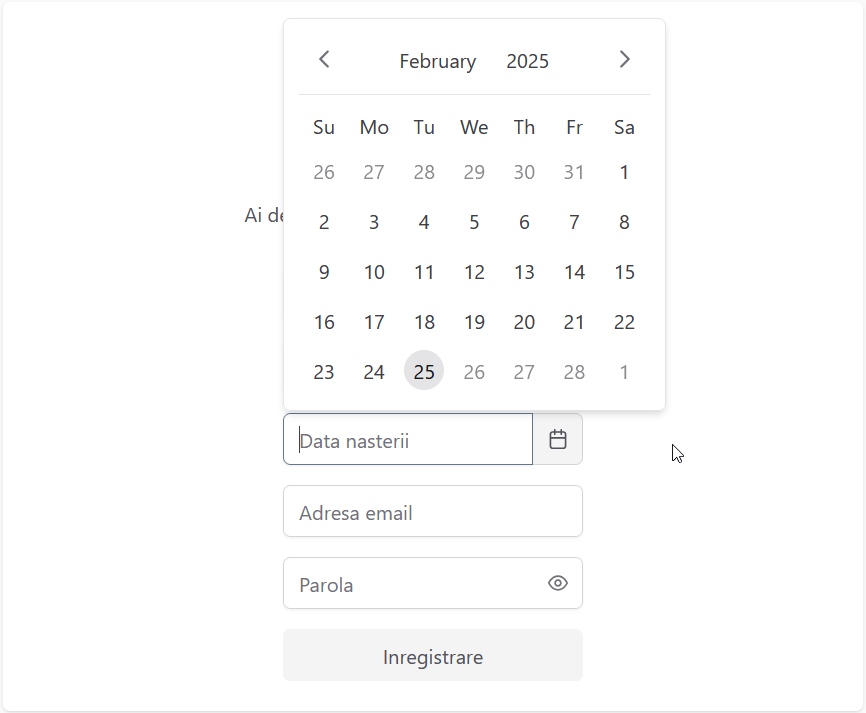
\includegraphics[width=\textwidth,height=0.8\textheight,keepaspectratio]{DatePicker.png}
  \caption{PrimeVue DatePicker component}\label{fig:datepicker}
\end{figure}

\FloatBarrier

As previously mentioned in~\ref{sec:techstack}, Vue also comes with other in-built tools that help create a well-working frontend. One of these tools is Vue Router, which was used to create the routes for the frontend. The student created a simple router that would allow the user to navigate between different pages. A navigation guard was used to protect the routes that required the user to be authenticated. An example of this can be seen below:

\begin{lstlisting}[caption=Vue Router Navigation Guard]
router.beforeEach(async (to) => {
  const authStore = useAuthStore()

  if (to.meta.requiresAuth) {
    await authStore.checkAuth() // Check if user is authenticated for protected routes
    if (!authStore.isAuthenticated) {
      return { name: 'Login' } // Redirect to login if not authenticated
    }
  } 
  // More code to handle other cases
})
export default router
\end{lstlisting}

Similarly, Pinia store was used to manage the authentication state of the user in the frontend. The store was then used by elements like the Navigation Guard to check if the user was authenticated before allowing them to access certain routes. An example of the store can be seen below:

\begin{lstlisting}[caption=Pinia Store for Authentication]
export const useAuthStore = defineStore('auth', () => {
  const isAuthenticated = ref(false)
  const user = ref(null)

  async function checkAuth() { // check if user is authenticated
    try {
      const response = await api.get('/me') // return user object if user is authenticated
      isAuthenticated.value = true // user is authenticated
      user.value = response.data.user
    }
    // More code to handle errors and no authentication
  }
  return { isAuthenticated, user, checkAuth }})
\end{lstlisting}

\subsection{Challenges}

One of the biggest challenges encountered in this sprint was the lack of experience using some of the frameworks and libraries used in the project. As such, this sprint's progress moved slower due to the learning curve that needed to be overcome first by reading the documentation and finding any guides/help online.

Another challenge was making decisions regarding different sections of the system, such as authentication, hashing algorithms, and others. Additional time was spent researching the best practices for each respective functionality \- analysing their advantages, disadvantages and ways to implement them in the current system.

\section{Sprint \#2}

The second sprint of this project was focused on building some of the smaller elements of the system, such as the ability to add vaccines, allergies and medications. The decision to start with the smaller elements was made to allow the student to get a better understanding of how the frameworks used in the project worked and to get a better understanding of how to structure the project.

\subsection{Adding Vaccines, Allergies and Medications functionality}

The student started by creating the schemas for the Vaccines, Allergies and Medications tables in the database. These tables were created in a similar way to the User table, using SQLModel schemas. Afterwards, the student created the endpoints that would allow the user to add, update, delete and view the data in these tables.

On the frontend side, the system used Vue's main strengths to enable a smooth developer and future user experience. Some of the strengths used were using Vue components to create reusable elemenets, such as a Vaccine Card that would be used to display the vaccines that the user had added. The card also used other Vue elements such as props and emits to pass data between parent and child elements and pass events, respectively. An example of the Vaccine Card can be seen below:

\clearpage

\begin{lstlisting}[language=HTML, caption=Vue Vaccine Card Component Example]
<Card class="w-full" :pt="cardStyles">
  <template #title>
    <span class="font-bold text-2xl">{{ name }}</span>
  </template>
  <template #subtitle>
    <div class="flex items-center justify-between">
      <div>
        <span class="font-bold">{{ provider }}</span>
        <span>{{ date_received }}</span> 
      </div>
      <div>
        <Button icon="pi pi-eye" class="p-button-rounded p-button-text"
          @click="emit('showFile', props.id)" v-if="hasCertificate"/>
        <Button icon="pi pi-ellipsis-h" class="p-button-rounded p-button-text"
          @click="toggle"/>
        <Menu ref="menu" :model="items" :popup="true" />
      </div>
    </div>
  </template>
</Card>  
\end{lstlisting}

The VaccineCard component can then be easily used in the main view:

\begin{lstlisting}[language=HTML, caption=Using VaccineCard Component]
<VaccineCard
  v-for="vaccine in vaccines"
  :key="vaccine.id" 
  v-bind="vaccine"
  :has-certificate="!!vaccine.certificate"
  @delete="deleteVaccine"
  @open-edit="openEditDialog"
  @show-file="showCertificate"
/>
\end{lstlisting}

\begin{figure}[htbp]
  \centering
  
\includegraphics[width=\textwidth,height=0.7\textheight,keepaspectratio]{VaccineCard.png}
  \caption{Vue Vaccine Card component}\label{fig:vaccinecard}
\end{figure}

\FloatBarrier

This format was used across the system to easily create reusable components that could be used in multiple places, making the system more modular and easier to maintain.

To make sure the data displayed in the frontend was always up to date, the frontend used Vue's reactivity system. This allowed the data to be automatically updated whenever any change was made to the data in the backend or frontend. Examples of the reactivity system in use can be seen below, with functions that add and delete vaccines from the frontend when called:


\begin{lstlisting}[language=HTML, caption=Vue Reactivity System]
// Will add a vaccine to the vaccines array, which will automatically 
// create a new VaccineCard element
const addVaccine = (vaccine) => {
  vaccines.value.push(vaccine)
}

// Will remove a vaccine from the vaccines array, which will 
// automatically remove the VaccineCard element
const deleteVaccine = (id) => {
  vaccines.value = vaccines.value.filter((vaccine) => vaccine.id !== id)
}
\end{lstlisting}

\subsection{File Uploads}

Another major feature that was implemented in the 2nd sprint was the ability to upload files. At the time of implementation, the feature was only to be used for uploading vaccine certificates, however it could be easily extended to other parts of the system, such as uploading health records or lab results.

To allow a proper upload of files, a new table was created in the database, called FileUpload. This table contained the file metadata, such as its name, size, type, path and others. Similarly, a new table for Allergy Severity was created to ensure consistency in the user uploads and to allow for easy filtering and searching of the data.

The updated ERD diagram with the new tables can be seen below in figure~\ref{fig:erd_s2}:

\noindent\begin{minipage}{\textwidth}
  \begin{center}
      \rotatebox[origin=c]{270}{
          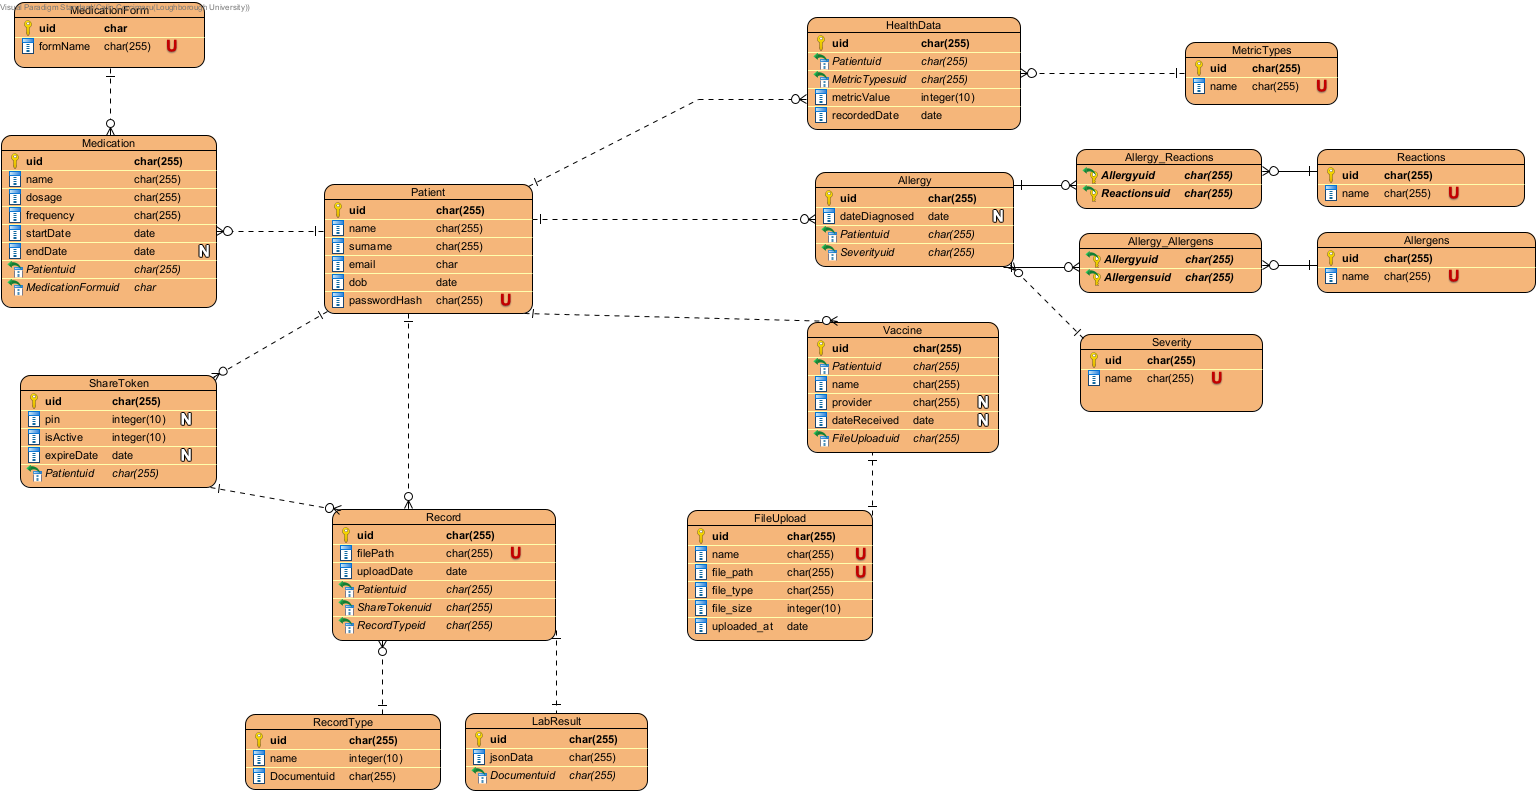
\includegraphics[width=0.95\textheight,keepaspectratio]{ERD_updatedS2.png}
      }
      \captionof{figure}{Updated Entity Relationship Diagram}\label{fig:erd_s2}
  \end{center}
\end{minipage}

To add more security to the system, the files were further encrypted before being stored in the database. AES was chosen as the encryption algorithm. Based on the articles analysed, it was consistently found to have the best balance between security and performance among other symmetric and asymmetric encryption algorithms \parencite{crypt1,crypt2,crypt3}. The choice to go with a symmetric algorithm was made due to its simplicity, as the key could be stored on the server-side in an environment variable, allowing the encryption and decryption of the files to be done on the server-side. This also allowed to avoid the issue of users losing access to their files if they lost their private encryption key, in the case of asymmetric encryption.

The encryption was done using the Fernet symmetric encryption algorithm from the cryptography library. Fernet uses AES-128 to encrypt the files. The key used to encrypt the files was stored in the environment variables and was generated when the system was started. In the interest of time, no rotation system for the key was implemented, however this would be a good feature to add in the future. 

The file upload process can be seen in figure~\ref{fig:fileuploadview} below. The file upload process was done in two steps. The first step was to upload the file to the server by using multipart form data. The next step would have the file be validated by checking its file type and size, then encrypted and stored in the file system and database. To access the files, the system used a new endpoint that would allow the user to download the file. The endpoint would take the file ID as a parameter and would stream the file to the user.

\begin{figure}[htbp]
  \centering
  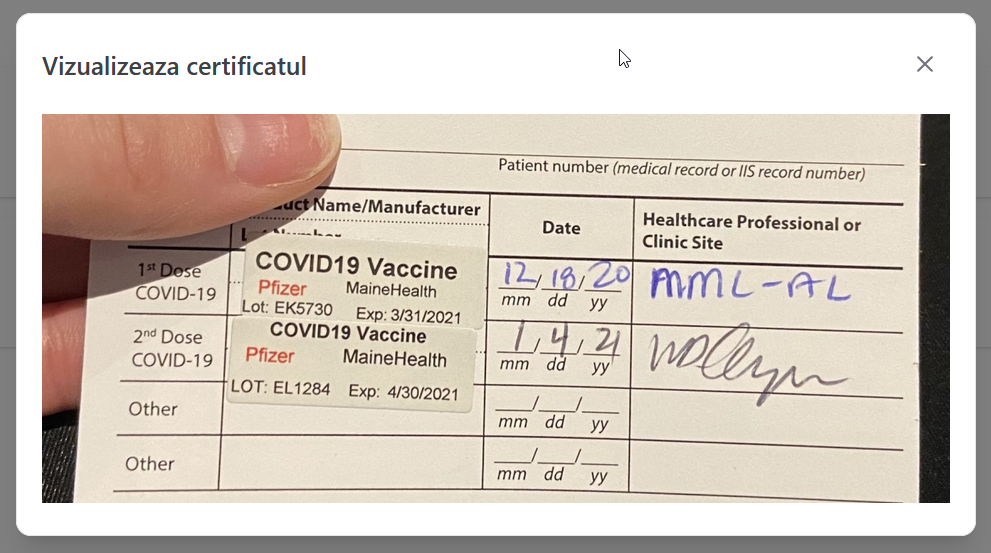
\includegraphics[width=\textwidth,height=0.7\textheight,keepaspectratio]{VaccineCertificate.png}
  \caption{Uploaded Vaccine Certificate}\label{fig:vaccinecertificate}
\end{figure}

\FloatBarrier

\begin{figure}[ht]
  \centering
  \subfloat[File Upload Sequence Diagram]{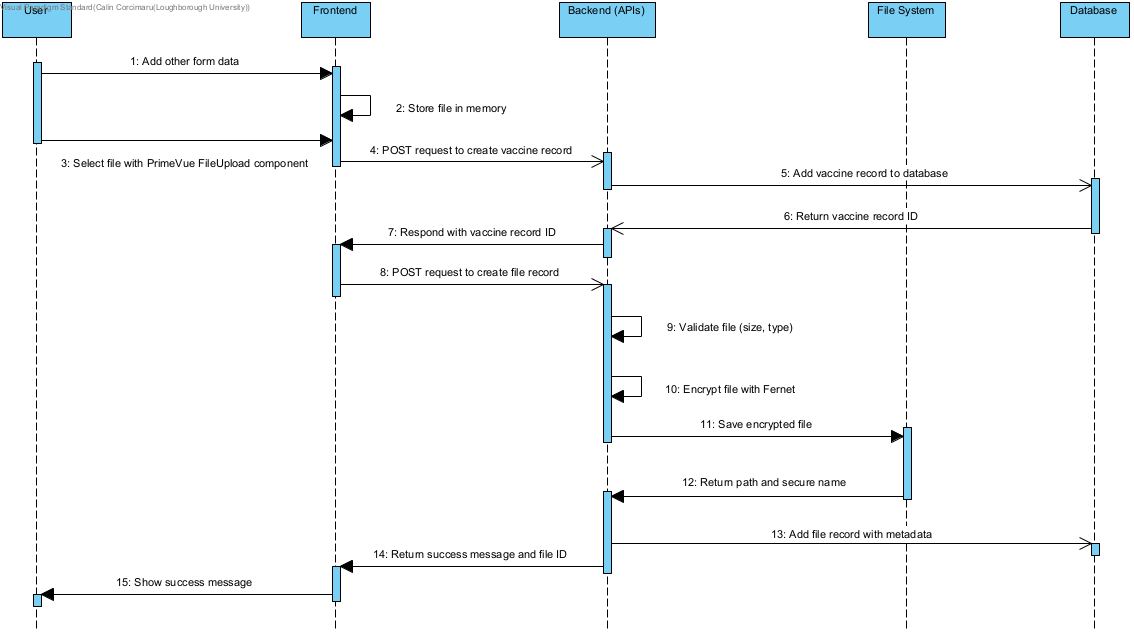
\includegraphics[width=\textwidth]{Sequence_FileUpload.png}\label{fig:seqfileupload}} 
  \\
  \subfloat[File View Sequence Diagram]{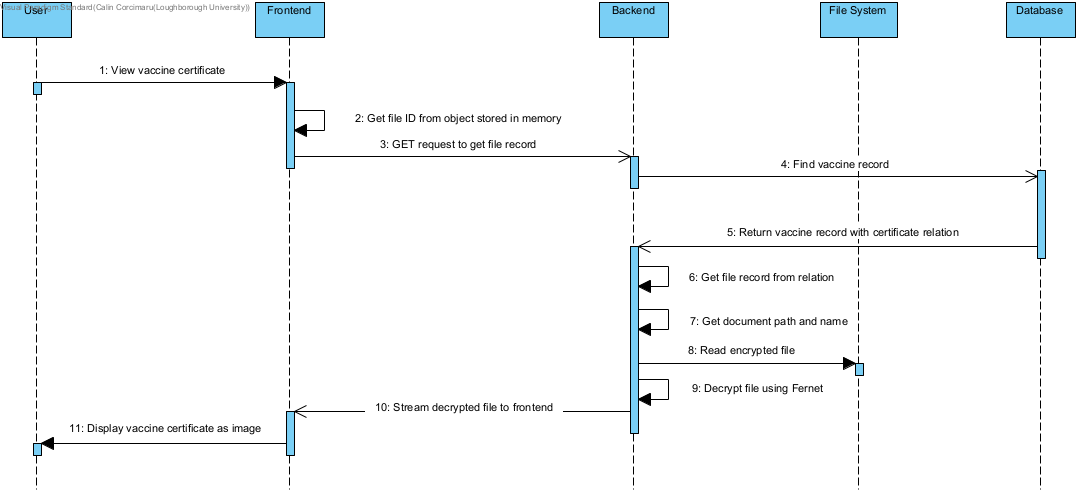
\includegraphics[width=\textwidth]{Sequence_FileView.png}\label{fig:seqfileview}} 
  \caption{Sequence Diagrams for File Upload and File View}\label{fig:fileuploadview}
\end{figure}

\FloatBarrier

The endpoint can be seen below:

\begin{lstlisting}[language=Python, caption=File Download Endpoint]
# Get a file by ID
@app.get("/files/{record_type}/{record_id}")
async def get_file(
  record_type: str,
  record_id: uuid.UUID,
  user_id: User = Depends(validate_session),
  session: Session = Depends(get_session)    
):    
  # Code to get the file record from the database
  
  async def get_data_from_file():
    with open(file_record.file_path, "rb") as f:
      encrypted_content = f.read()
      
    decrypted_content = decrypt_file(encrypted_content)

    yield decrypted_content
    
  return StreamingResponse(
    content=get_data_from_file(),
    media_type=file_record.file_type,
    status_code=status.HTTP_200_OK,
    headers={"Content-Disposition": f"inline; filename={file_record.name}"}
  )
\end{lstlisting}

Finally, the frontend was made with both mobile and desktop browsers in mind. This was achieved by using PrimeVue components and styling them with TailwindCSS. The system was also made to be responsive, so that it would look good on any screen size. Examples of the allergies page on both desktop and mobile can be seen below:

\begin{figure}[ht]
  \centering
  \subfloat[Desktop version]{%
      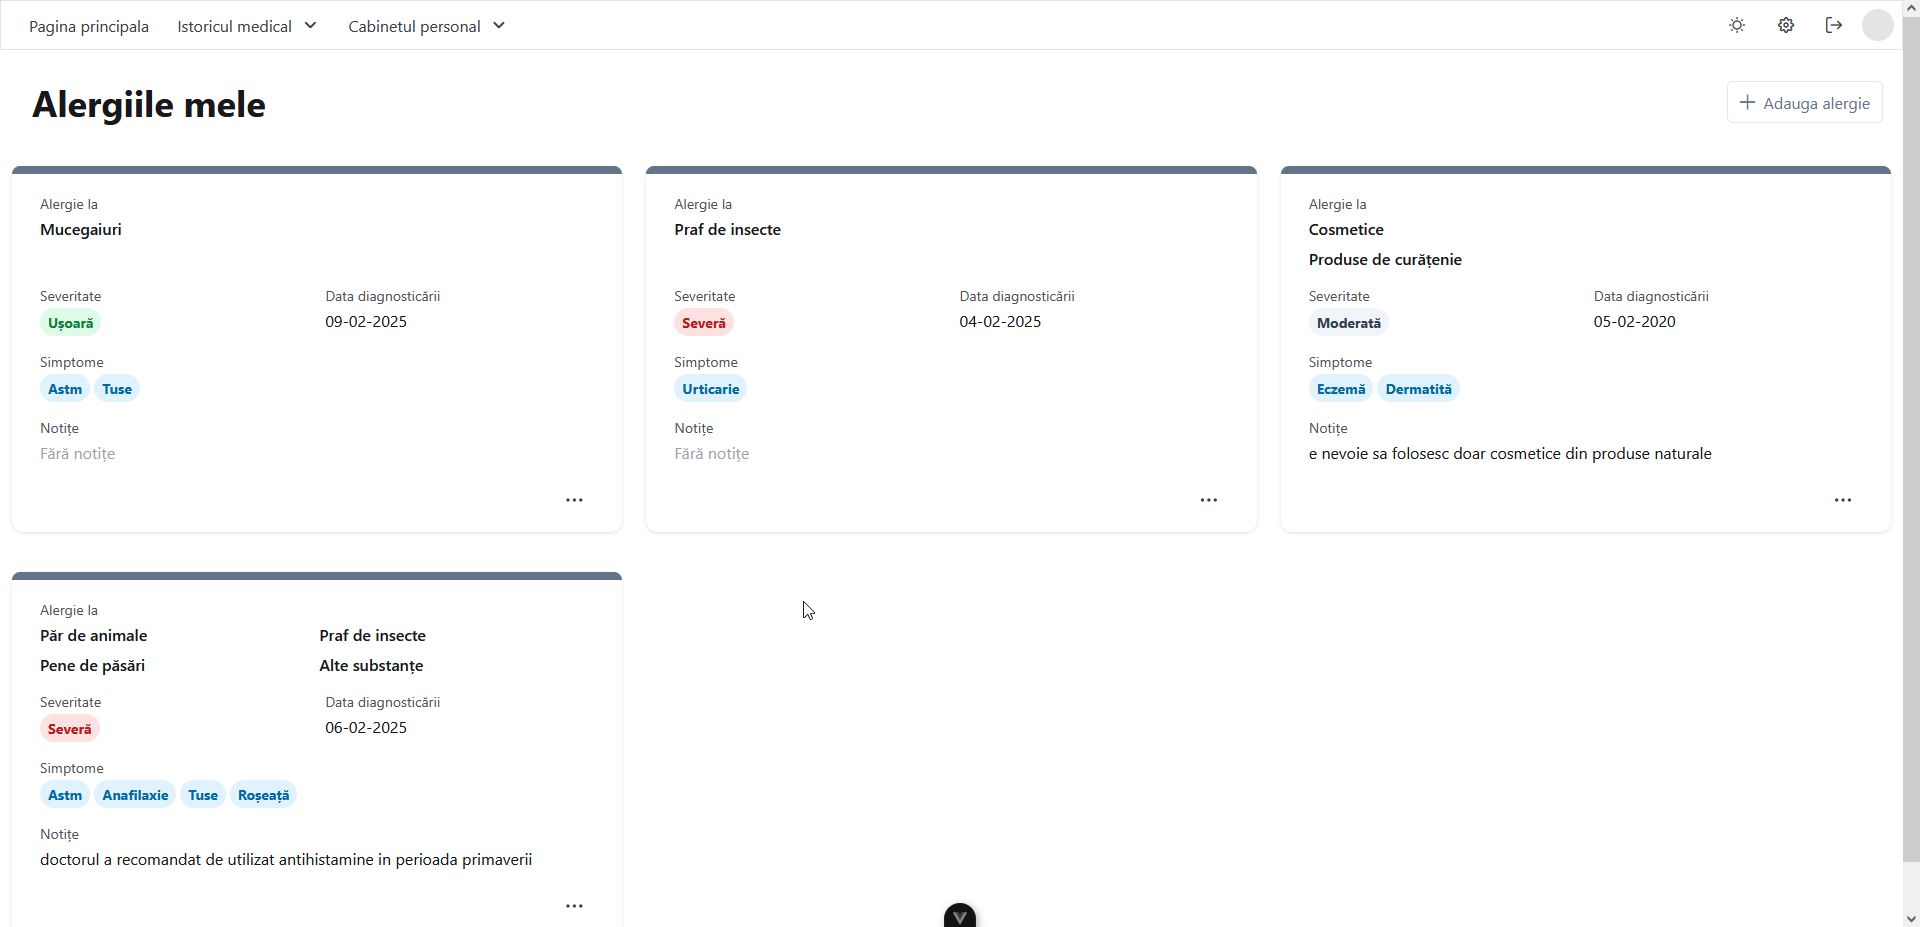
\includegraphics[width=\textwidth]{Desktop_AllergyView.png}%
  }
  \\[\baselineskip]
  \subfloat[Mobile version]{%
      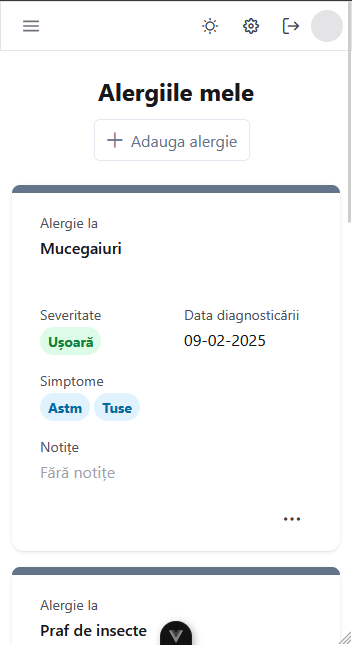
\includegraphics[width=0.4\textwidth]{Mobile_AllergyView.png}%
  }
  \caption{Desktop and Mobile version of the Allergies page}\label{fig:allergiespage}
\end{figure}

\FloatBarrier

\subsection{Challenges}

In this sprint, the main challenge was introducing the new features/functionality in the system, while ensuring they worked properly together with both the existing frontend and backend. For some features, there was a need to revise and change some of the existing code, such as the API endpoints and even the database schemas to accommodate the newly implemented changes. This added some additional complexity, as it was crucial to ensure the changes did not break any of the existing functionality, while allowing the new features to work as intended.

Another challenge was understanding how some of the newly implemented features worked, such as the file upload system. It is important to note that the student had no previous experience implementing any file upload functionality, so extra time and work was dedicated to ensure the relevant documentation was studied and then implemented correctly.

Finally, due to lack of time and poor initial planning because of the complexity of the system, some of the features intended for this sprint had to be moved to the next one. Some examples include the health data section and also the main dashboard parts for vaccines, allergies, medications and health data. 

These changes and challenges show that undertaking a more agile approach to the project was beneficial, as the project embraces change and allows for more flexibility in the development process.

\section{Sprint \#3}

\section{Sprint \#4}

\section{Sprint \#5}

\section{Sprint \#6}